\section{NLP}
\subsection{Introduction}

In a computerised learning course, tailoring the course contents to the specific pre-existing knowledge of an individual learner allows the learning material to be covered more efficiently by focussing on subjects that are not yet well understood as opposed to subjects that the learner (user) is likely to know well. Knowledge estimation deals with the question of parametrising and modelling the knowledge about various topics (items) on a per-user basis. 

In this report, we describe a computational method for estimating the overall second-language vocabulary of users, based on answers to a small set of trial words that the users attempt to guess. By implementing a simplified version of Deep Knowledge Tracing \cite{DBLP:journals/corr/PiechSHGSGS15}, we show that by predicting the knowledge of individual items on a per-user basis using a sequence of previous guesses, we can develop an accurate estimation procedure for the overall knowledge of the user.

We achieve this by compressing the sparse and variable-length guess sequences into a fixed-size representation using a recurrent neural network (RNN) and furthermore mapping this small fixed-size representation into a vector that can be interpreted as distinct per-item knowledge likelihoods.

This report is organized as follows: in the first section, we review the mathematical background of the problem of knowledge estimation and present a statistical overview of the data. In the second section, we discuss the details of the RNN model that will be used to estimate the user knowledge and compare it with other models. In the third section, we summarize the studies that were made in optimizing the RNN model, analyse the results and discuss possible improvements that could be made to the model.

\subsection{Problem statement and data description}

\subsubsection{Knowledge tracing}
The problem of knowledge estimation can formally be stated in the following way. We have a set of items, indexed by $n = {1, 2, \dots, N}$, for which users, indexed by $m  = {1, 2, \dots, M}$ provide guesses which can be correct or incorrect, denoted by $g_{nm}=\{1, 0\}$. Therefore on a per-user basis, the guess data form a sequence $S_m = [(n_1, g_1), \dots, (n_i, g_i), \dots, (n_T, g_T)]$ where $T$ is the number of guesses a user has made. Knowledge of a specific user can then be succinctly written as $\vec{g} = (g_1, g_2, \dots, g_M)$. We assume that we have no control over the order in which items are presented to the user, in general, the sequence may contain guesses in an arbitrary order, possibly with gaps between the successive indices $m_i$ and $m_{i+1}$. The items themselves may be arbitrary, but in our case, they always represent word pairs, asking the user to guess a word in their target language based on an explanation in their source language. We use the term lexical unit (LU) to denote such word pairs. An example of a LU for the word *conseil - advice* can be seen on \cref{fig:lu_example}.

These data can be represented as a $(N \times M)$ matrix $G = (g_{nm})$, with $N$ being the total number of users and $M$ the total number of items. In general, due to the specifics of the way the questions are posed to the users, this matrix is sparsely filled, as can be seen on \cref{fig:user_data}.

\begin{figure}[ht]
\centering
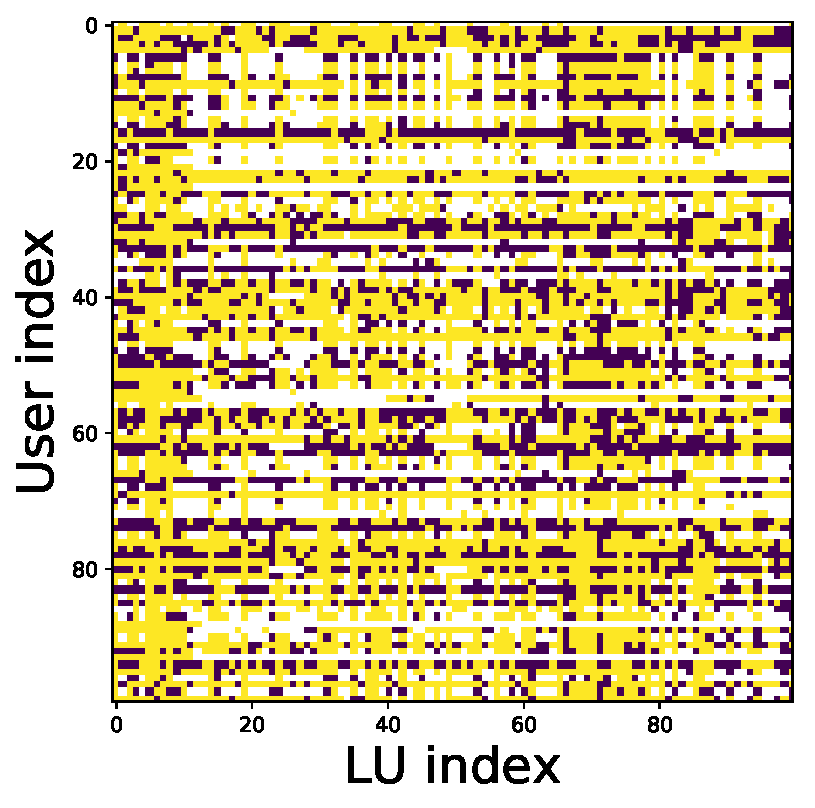
\includegraphics[width=0.5\linewidth]{figures/lingvist/user_data.pdf}
\caption{Guess data for the first 100 users and the first 100 LUs. Correct guess attempts are shows as yellow pixel, incorrect attempts are violet. Cases where data was not available are white. We show a subset of the whole user population and the item set.} 
\label{fig:user_data} 
\end{figure} 

The task of knowledge estimation is then to predict the guess probabilities $\vec{g}$ for all items for a individuals user, given a short ($\sim5\%$ of the total) subsequence of that user's guesses.

We stress that the guess probabilities of items may well be related to each other, for example some words can be of similar meaning or difficulty, hence we wish to model the full probability distribution $p(\vec{g})$. However, we do not have an explicit labelling of which items are related and we hope to capture the essential properties of the knowledge probability by using the data directly.

\begin{figure}[ht]
\centering
\begin{tabular}{cc}
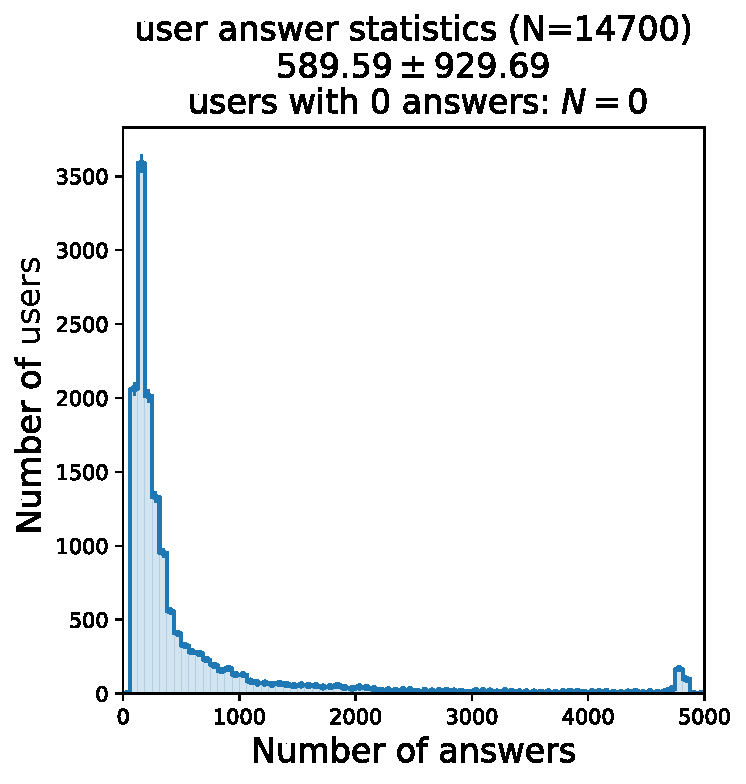
\includegraphics[width=0.4\linewidth]{figures/lingvist/user_answer_distribution.pdf} &
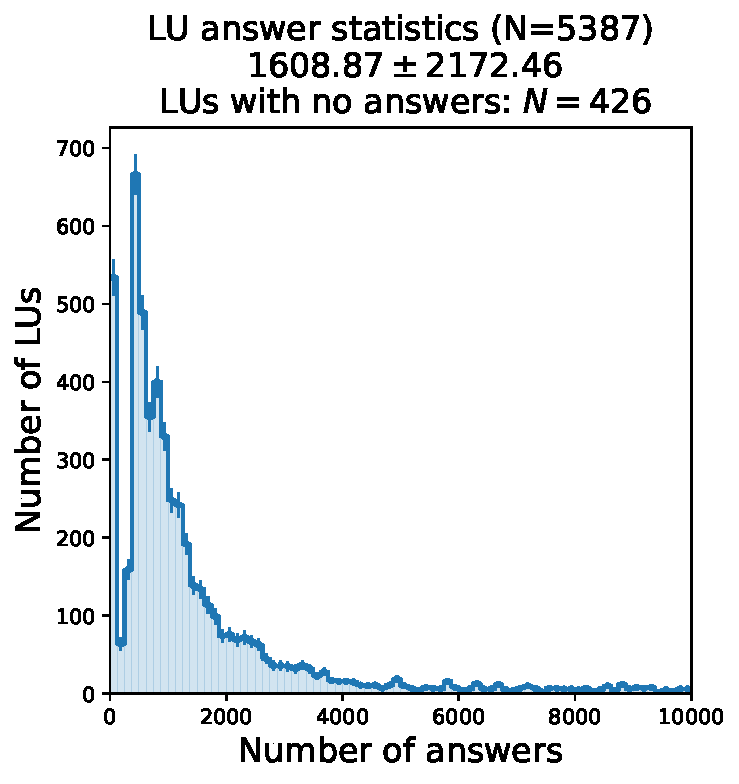
\includegraphics[width=0.4\linewidth]{figures/lingvist/lu_answer_distribution.pdf} \\
\end{tabular}
\caption{On the left, we show the distribution of users by number of answered LUs. We have required that a user has answered at least 100 LUs. On the right, we show the corresponding distribution of LUs by number of answers from users. Currently, LUs have not been filtered, hence the whole course is considered.} 
\label{fig:user_lu_distribution} 
\end{figure} 

\subsubsection{Data}
We use data from roughly 15000 users from the English to French course at Lingvist, requiring that users have answered at least 100 words. The course consists of roughly 5400 individual LUs. Overall, an average user has answered about 590 LUs and an average LU has about 1600 answers, however, the distributions have significant non-Gaussian tails, as can be seen on \cref{fig:user_lu_distribution}. We have also validated the model on several different language pairs and have seen that the results are broadly replicable.

The problem as stated here is well known in literature as matrix completion\cite{candes2009exact}, where the task is to discover hidden or latent variables that would allow the unspecified elements of a matrix to be estimated based on assumptions about rows or columns being sampled from a common distribution. Such problems are typically solved with some combination of collaborative filtering and matrix factorization. However, as we may also want to model time-dependent behaviour of the estimated knowledge, we seek a more generic solution to the problem that would make it possible to add arbitrary information about users and guesses and derive the appropriate model without much expert knowledge.

\subsection{Model description}

\subsubsection{Baseline models and performance evaluation}

Here we describe the baseline models that will be used as reference implementations. The simplest model for predicting the prior knowledge rate of words would simply be to assume that any user is an average user and each word with index $n=1 \dots N$ has a probability $p_n$ of being known by any user, where the probability is simply estimated by computing the ratio of correct to all guesses of this word by all users. Clearly this does not allow the learning experience to be tailored, but it is a reasonable first guess about the user in the absence of other data.

As the user proceeds through the course, their guesses will allow us to update our estimation of their knowledge in a Bayesian framework. In general, Bayesian Knowledge Tracing \cite{corbett1994knowledge} has been shown to perform at least as well as the best machine-learning based models, however, such models require considerable domain knowledge and manual item labelling to be used successfully\cite{khajah2016deep}, thus we investigate supervised neural networks as a possible solution.

In order to measure how well a model is able to predict the known items, we need to establish a set of metrics. In particular we use the number of correctly predicted items that the user actually knows (true positives) and the number of items incorrectly predicted to be known (false positives). Thus, we effectively treat the problem as binary classification with each guess attempt being an independent trial of equal weight. 
We use these true and false positive rates to construct the receiver operating characteristic area-under curve (ROC AUC) as an overall average performance indicator. Such a metric considers all trials as equal, meaning it is tuned to measure the performance of the model on the same distribution of words that we use to train it with. An alternative would be to treat each word, regardless of how many guesses have been made for it, as equal. We refer to this later as the LU-weighted case.

\subsubsection{RNN-based model}
Since we may want to make predictions continuously as the user progresses through the course, the model should be able to deal with sequence data of varying length. This leads us to consider recurrent neural networks as a possible model architecture. In particular, inspired by the Deep Knowledge Tracing framework\cite{DBLP:journals/corr/PiechSHGSGS15}, we use a Long Short-Term Memory (LSTM)\cite{gers1999learning} architecture to summarize a guess history of arbitrary length as a vector of fixed length. Effectively, this means that on a per-user basis, the questions that are used to estimate the knowledge of a particular user are fed one-by-one into the LSTM cell, which creates a fixed-size representation of the user's knowledge, which is then mapped into the output space as $\vec{g}$. Between the LSTM layer and the output layer, we use a number of densely connected layers interleaved with dropout regularization in order to approximate the knowledge decoding transformations.

We use a RNN as opposed to a dense network working on a fixed-size input in order to be able to give accurate estimations of the user's knowledge before the full sequence is seen. Nevertheless, the RNN needs to be trained with a fixed input size $N_{\mathrm{sequence}}$.

The parameters to optimize in the model are the input, output and forget gate weights and biases and the weights of the dense layers connecting the LSTM output to the final output vector.

As hyperparameters, we optimize the size of the LSTM layer, the number and size of the intermediate dense layers and the amount of dropout that is applied.

Care must be taken when computing loss function that is minimized in optimizing the weights. Since for any user, the known guess vector $\vec{g}_\mathrm{true}$ is sparse, we must compare only those prediction values that are specified. Technically, we implement this by propagating the boolean mask of available answers as an auxiliary input and compute the binary cross-entropy loss only over available answers.

\subsubsection{Model architecture}

In order to feed the $(\mathrm{question}, \mathrm{answer})$ pairs into the LSTM, we need to define an appropriate numerical representation of the questions. As the set of all possible questions is known at training time, we could simply consider each question as a unique symbol that can be embedded into a real vector space by some appropriate function. Each question is also a word, or more precisely a word pair in the source-target languages, thus we could use an existing word embedding such as \verb|word2vec|\cite{mikolov2013efficient} or \verb|GLOVE|\cite{pennington2014glove} defined on a large corpus of text. However, a predefined word embedding would limit the model to only be useful for word-based questions, excluding the possibility of using data from other types of activities without additional steps. Another option would be to derive the embedding directly as part of the neural network optimization procedure. We attempted this direct embedding and it gave generally good results, but was not chosen due to practical reasons described below.

Instead of an optimized embedding described above, we may use random vectors to represent the questions. Using compressed sensing, we can reconstruct any d-dimensional k-sparse signal using at most $\simeq k\log d/k$-element random vectors\cite{baraniuk2007compressive}. In our case, the dimensionality is the number of individual items or symbols ($N$) that we want to represent and the sparsity is $k=1$ for a one-hot encoding, thus, a uniform random vector of length 4-5 would be sufficient to represent all the words in the whole course.

We choose the random vector approach, as we can easily use the unique \verb|UUID4|-based database identifiers as encoding vectors by mapping the 128 random bits to 16 random 8-bit floats in the range $[-1, +1]$. This way, we don't need to go through the additional trouble of keeping track of item to representation associations throughout the lifetime of the product, as they are always uniquely specified just by the item's identity.

For each user, we take up to a fixed number $N_{\mathrm{sequence}}$ of guesses as the input and predict their full knowledge vector $\vec{g}$. The model is thus the following:

\begin{gather*}
\mathrm{sequence} = [(\mathrm{representation}, \mathrm{guess}), (\mathrm{representation}, \mathrm{guess}), \dots] \rightarrow \\
\rightarrow \mathbf{LSTM} \rightarrow \mathrm{encoded\ knowledge} \rightarrow \\ \rightarrow \mathrm{dense} \rightarrow \cdots \rightarrow \mathrm{dense} \rightarrow \\
\rightarrow \mathrm{dense\ output\ with\ sigmoid\ activation} \rightarrow \vec{g} 
\end{gather*}

We train the model with minibatches of 100 users for about 20-100 epochs with the Adam optimizer using early stopping.

\subsection{Results}

\subsubsection{Optimization studies of the RNN model}

In general, the model performance has only a mild dependence on the choice of hyperparameter values. Nevertheless, we scan the hyperparameters by computing a cross-validated mean AUC at each point in a 5-dimensional space, consisting of the size of the LSTM layer, the size of the intermediate dense layers, the number of intermediate dense layers, the amount of dropout and the learning rate. We find that the hyperparameter scan prefers the encoding by the LSTM to be rather small, around 32 to 64 units, and the intermediate dense layers are preferred to be small (128-256) and deep (3-4 layers). The final optimized loss function is shown on \cref{fig:loss}.

\begin{figure}[ht]
\centering
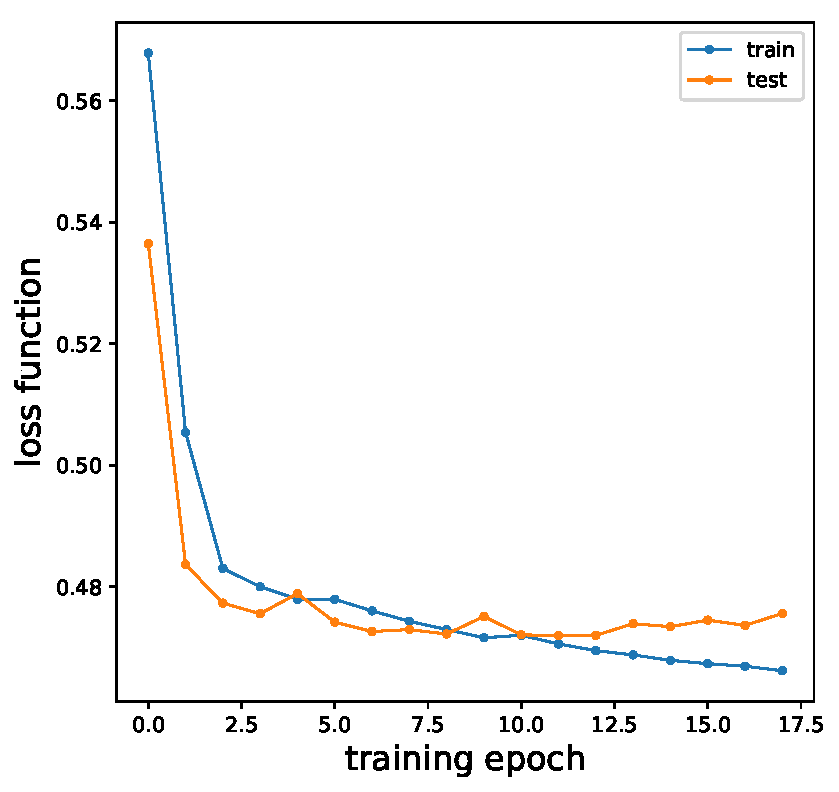
\includegraphics[width=0.5\linewidth]{figures/lingvist/loss.pdf}
\caption{The loss function of the final optimization of the model. The loss on the training set is shown in blue, the validation set in orange.} 
\label{fig:loss} 
\end{figure} 

One of the free parameters of the model is the length of the input guess sequence. We have studied how this affects the performance of the model by retraining the model on the same dataset, selecting up to $N_{\mathrm{guess}}$ guesses for each user. As expected, the model performs better if more information is provided about the user. We observe a roughly linear relationship between the AUC and the guess sequence length, as can be seen on \cref{fig:seq_length}.

\begin{figure}[ht]
\centering
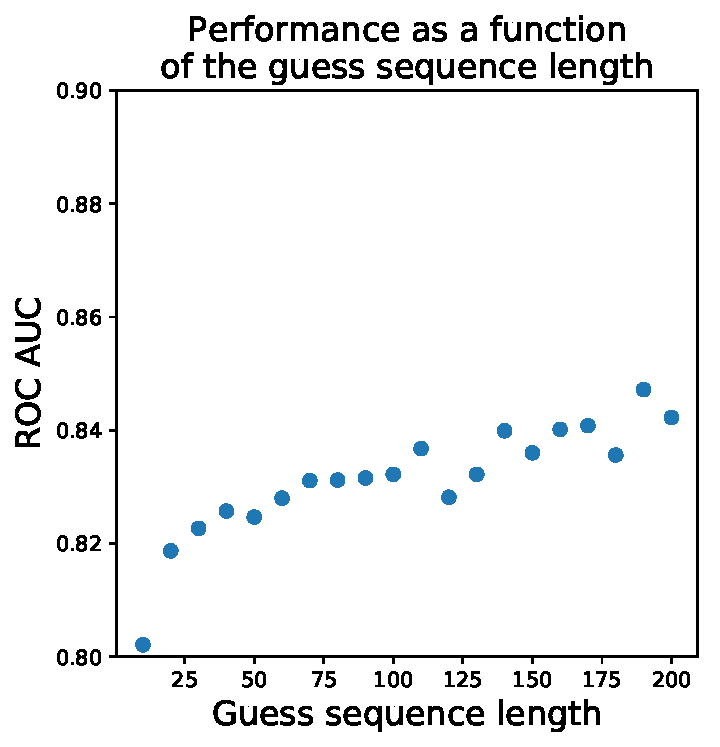
\includegraphics[width=0.5\linewidth]{figures/lingvist/seq_length.pdf}
\caption{Performance of the model as a function of the guess sequence length. For each point, we use only up to $N_{\mathrm{sequence}}$ guesses from all users as the input to the model. The model is trained from scratch on the full dataset and evaluated in the same way for all cases.} 
\label{fig:seq_length} 
\end{figure} 

We also study how the amount of training data affects the performance of the model.

\subsubsection{Discussion}

We show the average performance of the RNN model on \cref{fig:roc}, comparing it to the average user model. In general, we see that the neural-network based model is more accurate than the average model, with the average true positive rate improving from 0.38 to 0.54 at an average false positive rate of 0.1.

\begin{figure}[ht]
\centering
\begin{tabular}{cc}
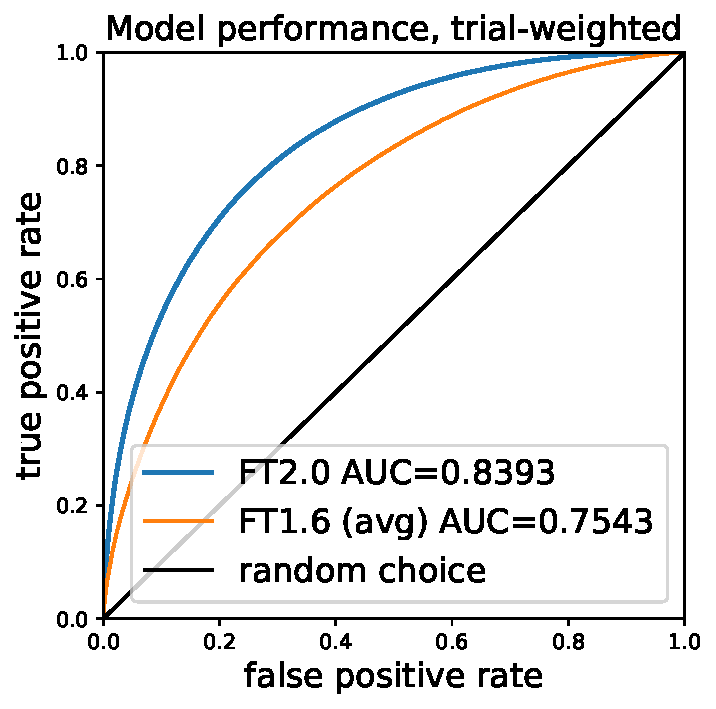
\includegraphics[width=0.4\linewidth]{figures/lingvist/roc_trial.pdf} &
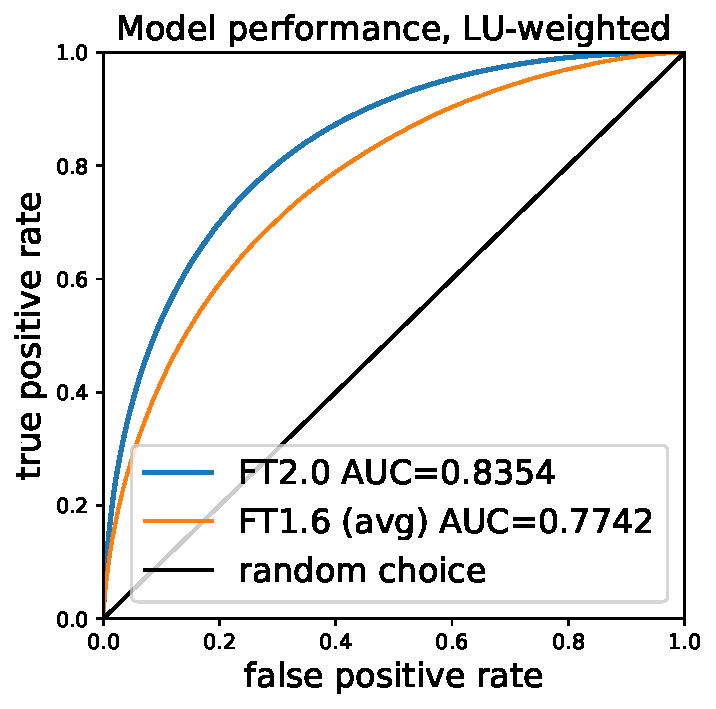
\includegraphics[width=0.4\linewidth]{figures/lingvist/roc_lu.pdf} \\
\end{tabular}
\caption{Overall average performance of the model, as characterised by the receiver operating characteristic (false positive to true positive rate curve) area under curve (ROC AUC). On the left, we show the average treating all trials equally, on the right, the average by weighting trials such that each word is treated equally. We see that the RNN model (blue) outperforms the average model (orange).} 
\label{fig:roc} 
\end{figure} 

On \cref{fig:user_lu_correct_rate} we see that the per-word and per-user correct rates are also reproduced to a good degree by the model. We can see that the correct rate for users and LUs with a low (high) average correct rate are slightly under (over) estimated. This could result from the model not having enough counterexamples to sufficiently learn the probability distribution $p(\vec{g})$ for very simple or hard words and users with very low or high correct rate. We take this as an example that the model is able to summarize the user and LU population and approximate some useful first-order statistics.

\begin{figure}[ht]
\centering
\begin{tabular}{cc}
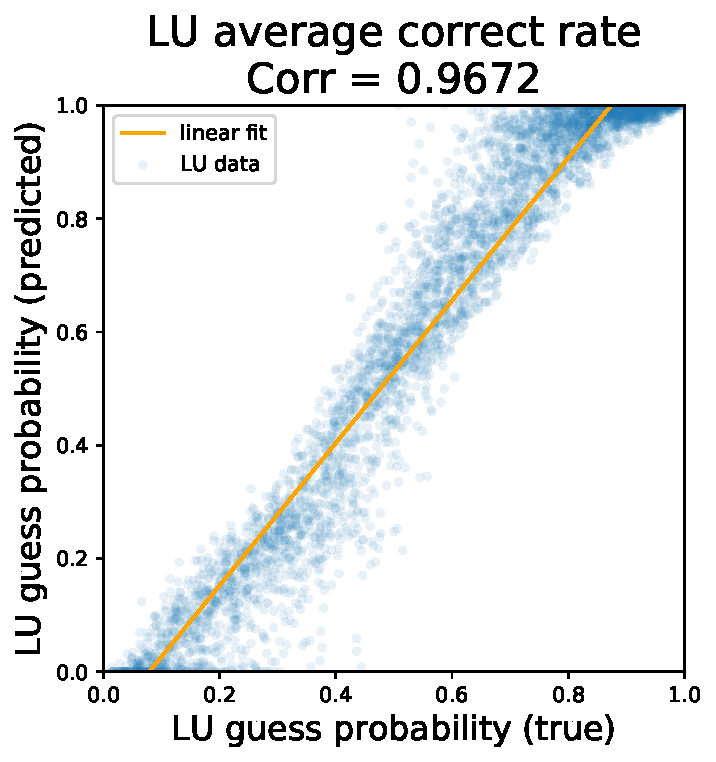
\includegraphics[width=0.4\linewidth]{figures/lingvist/lu_correct_rate.pdf} &
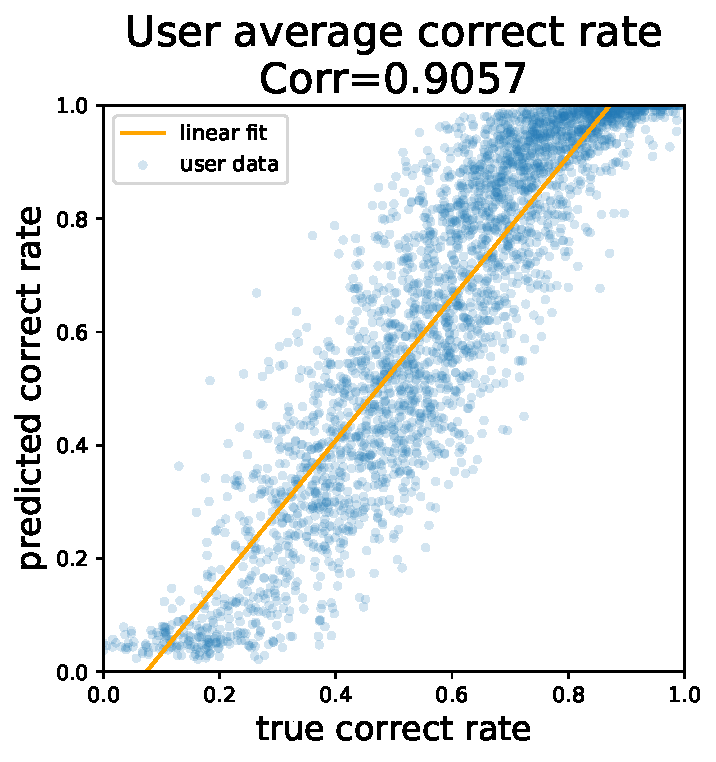
\includegraphics[width=0.4\linewidth]{figures/lingvist/user_correct_rate.pdf} \\
\end{tabular}
\caption{Predicted vs. true average guess rate by word (left) and user (right). We see that the model performs best for words which have a true correct rate around 50\%, with slight underestimation at low correct rates and overestimation at high true correct rates.}
\label{fig:user_lu_correct_rate}
\end{figure}

Additionally, on \cref{fig:lu_roc_prio} we see that the overall performance of the model is strongly dependent on how many guesses a given word has, with the average ROC AUC dropping significantly for rarer words. This performance degradation is expected, as we can see from \cref{fig:user_lu_distribution} that the number of answers per word drops significantly deeper in the course, reflecting that this model was trained treating each trial equivalently. With increasing guess statistics, it may be worthwhile to investigate a re-weighting of the trials such that words that have fewer trials have a higher weight and would thus still be optimized for in the training. This trend also introduces a natural cut-off in terms of when the predictions from the model are no longer considered reliable.

\begin{figure}[ht]
\centering
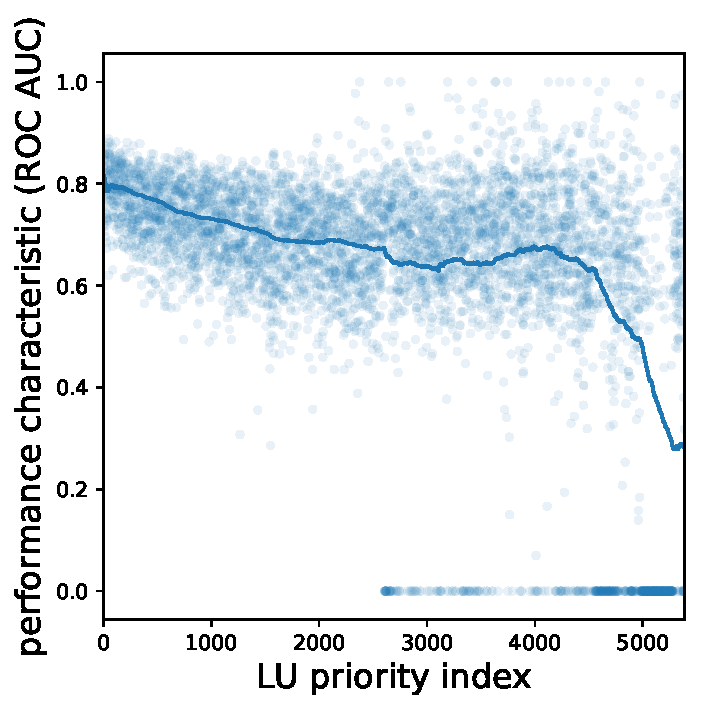
\includegraphics[width=0.5\linewidth]{figures/lingvist/lu_roc_prio.pdf}
\caption{The performance characteristic (ROC AUC) as a function of lexical unit priority index. The priority index is a monotonously growing index that roughly corresponds to the order in which words are shown to users, with lower indices being shown earlier and more often.}
\label{fig:lu_roc_prio}
\end{figure}

We see on \cref{fig:lu_roc_guess_proba} that the performance of the model is broadly similar over a wide range of word difficulties. For words that are very easy or difficult, the variance in the trained model is considerable.

\begin{figure}[ht]
\centering
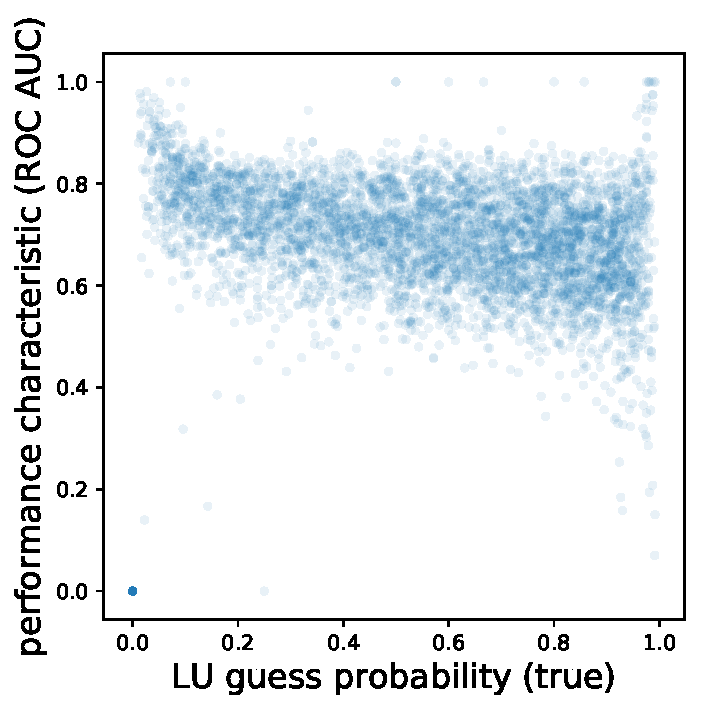
\includegraphics[width=0.5\linewidth]{figures/lingvist/lu_roc_guess_proba.pdf}
\caption{The performance of the model on a per-word basis as a function of the guess probability (prior difficulty) of the word. We see that for words with very high or low guess probability, the variance of the model is significant, resulting from few training examples.}
\label{fig:lu_roc_guess_proba}
\end{figure}

We have also investigated the prediction uncertainty arising from the model. In particular, for a word that is predicted to be known at a knowledge level of $p=0.9$, how certain is the model of this prediction and how much would it vary if the inputs changed slightly? For neural networks, it has been shown that using dropout in the evaluation phase is a good approximation for the inherent prediction uncertainty \cite{gal2016dropout}. On \cref{fig:uncertainty}, we can see the evaluated uncertainty of the guess probability using 10 dropout rounds, compared to the data. It is interesting to see that the 95\% confidence interval around the predicted mean covers the data, however, the predicted mean generally trends lower than the true guess probability.

\begin{figure}[ht]
\centering
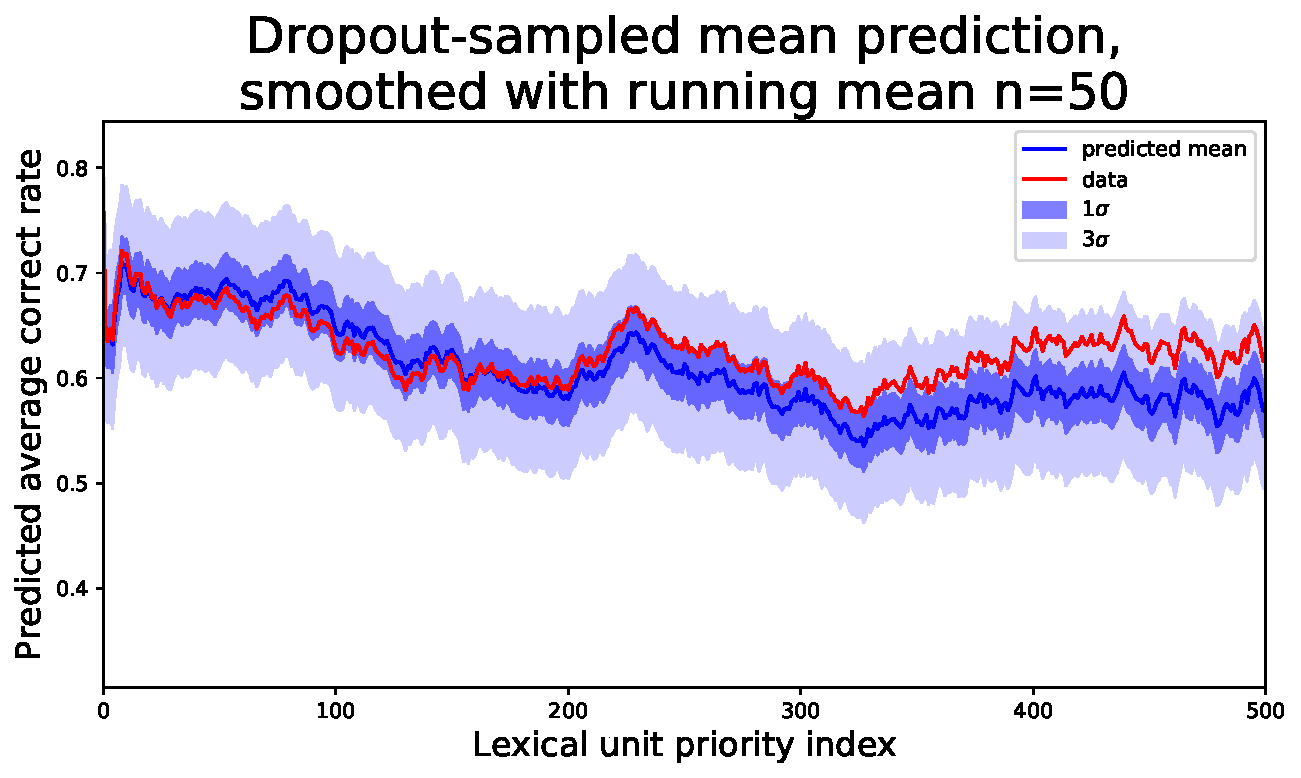
\includegraphics[width=1.0\linewidth]{figures/lingvist/uncertainty.pdf}
\caption{The predicted (blue) and true (red) guess probability as a function of LU priority index. We see that the prediction is generally sufficient, but trends somewhat lower than the data.}
\label{fig:uncertainty}
\end{figure}

Additionally, we have studied how the amount of training statistics affects the performance of the model. Interestingly, we see that with even as few as 1000 users, the model is able to approximate the knowledge characteristics of an average user. In general, adding more data improves the performance more significantly for words for which there are very few answers provided, as can be seen on \cref{fig:statistics}. Adding more data improves the model performance, especially for words with very low answer rates.

![The effect of the amount of training data on the model performance We investigate 3 cases: 1000 users, 5000 users, 15000 users (full dataset) and plot the performance characteristics of the model (ROC AUC), averaged over words that have a certain fraction of users providing answers.\label{fig:statistics}](figures/statistics.pdf){ width=50% }

\subsubsection{Future work}

As possible future improvements, extending the information in the word feature vector beyond a random representation may prove to be a simple way to improve the performance of the model. Additionally, Deep Knowledge Tracing was originally conceived for time-dependent knowledge modelling and the current framework is naturally amenable to predicting guess sequences in time. Furthermore, the current model works only on a single language pair, but it could easily be extended to multiple simultaneous languages by adding language data to the source representation vector and decoding the internal knowledge representation into different target spaces. This would allow training a single model on all language pairs simultaneously, which could help bootstrapping new courses that don't yet have enough answer data.

\subsection{Summary}

We have shown that by formulating the problem of predicting existing knowledge as a sequence-to-vector binary classification problem, recurrent neural networks present a simple and flexible solution applicable to a wide variety of cases. A single model architecture is able to predict knowledge probabilities of thousands of words based on just a small amount of randomly chosen guesses. The RNN model is easily extensible, should more information about words or users become available. In particular, we see extension to predicting knowledge in multiple languages simultaneously as a possible future improvement. 

Having produced a model capable of estimation, it is interesting to study the explanatory factors of that model. In general, explaining the decisions or predictions of complex "black box" models is an open research topic. Recently, locally interpretable linear models have been proposed as a way of explaining the features a model makes use of for particular predictions\cite{ribeiro2016should}. We have used the method to validate our trained model on a few examples and see that it uses guess information in an intuitively correct way, as can be see on \cref{fig:lime}.

\begin{figure}[ht]
\label{fig:lime}
\centering
\begin{tabular}{cc}
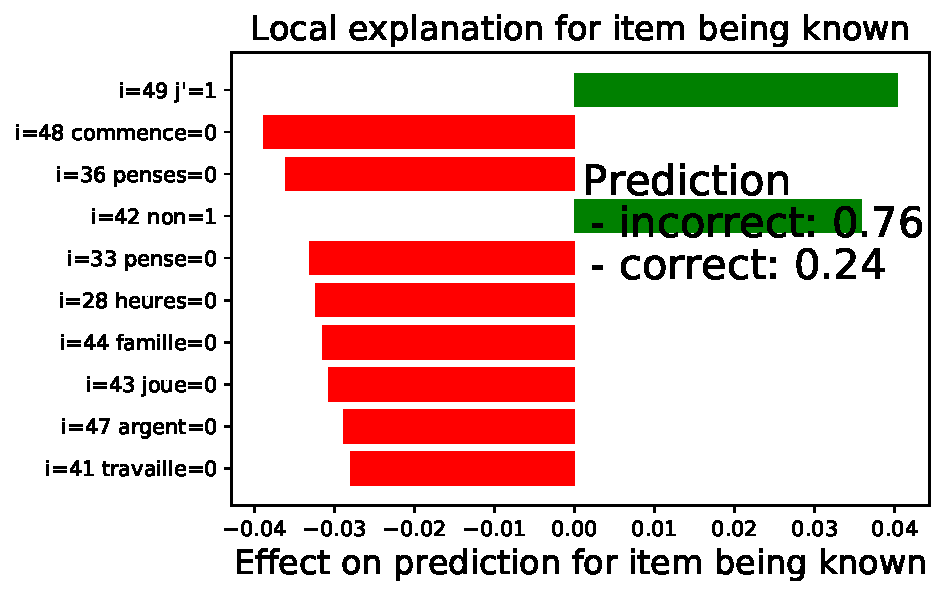
\includegraphics[width=0.4\linewidth]{figures/lingvist/lime_pos.pdf} &
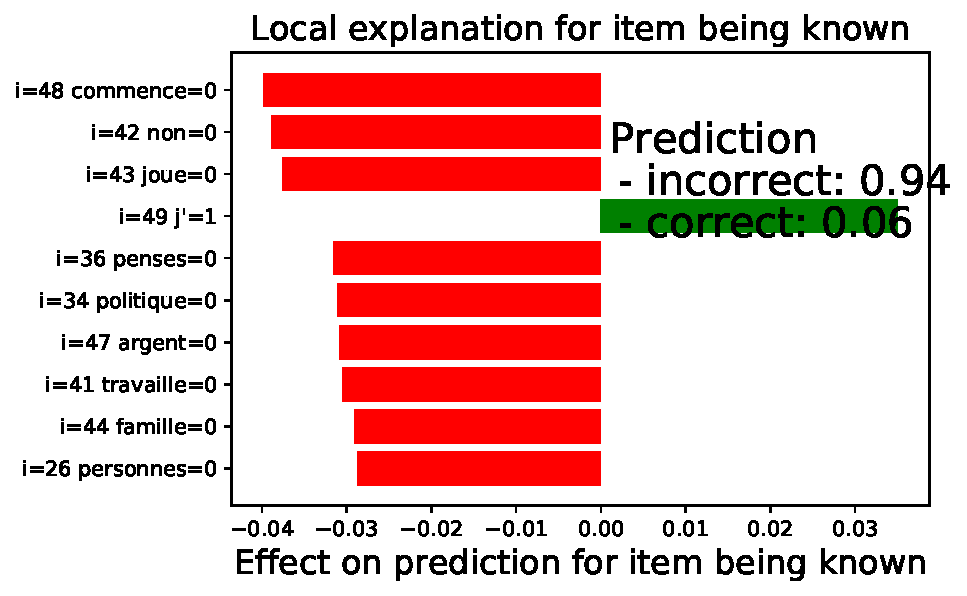
\includegraphics[width=0.4\linewidth]{figures/lingvist/lime_neg.pdf} \\
\end{tabular}
\caption{Local explanations for a word that was known (left) and not known (right). We see that incorrect guesses ($=0$) tend to affect the prediction in a negative way, whereas correct guesses ($=1$) tend to reinforce the knowledge, as would be expected.}
\end{figure}
